\chapter{解析}\label{analysis}
測定データを用いてどのように荷電粒子の飛跡の推定を行ったかを説明する。

\section{解析に用いたデータ}
表\ref{tab:analyzed_data}に示すようにトリガーレート15\ cps, データ取得時間約260時間, 取得イベント数12054470イベントのデータを解析に用いた。
\begin{table}[H]
    \centering
    \caption{解析に用いたデータ}
    \label{tab:analyzed_data}
    \begin{tabular}{|c|r|}
        \hline
        トリガーレート & 15 cps    \\ \hline
        取得時間       & 約260時間 \\ \hline
        イベント数     & 12054470  \\ \hline
    \end{tabular}
\end{table}

\section{しきい値の設定}\label{sec:anal:threshold}
測定によって得られたデータは各チャンネル毎に12bit (4096段階) の強度を持っている。ここでは12bitを0から4095までの整数で表すことにし, その値のことを ADC value と呼ぶ。
ADC value はMPPCから得られた信号をEASIROCが増幅, 整形しAD変換を行うことで得られた値である。
ADC value はMPPCからの信号強度, すなわち荷電粒子がシンチレータに渡したエネルギーに比例している量であるのでADC valueに適切なしきい値を設けることでシンチレータ毎に荷電粒子が通過したかどうかを判別できる。
シンチレータがエネルギーを受け取らなかった時のADC value は本実験で用いたEASIROCにおいては典型的に800付近であったため(TDOO: ペデスタルだけのhistの絵), ADC value 800付近からある程度離れた値をしきい値とすることにした。
具体的には表(TODO: threshold-effeciencyの曲線)のようにADC value のしきい値を800から1500まで1刻みで変更した時の検出効率を計算し, チャンネル毎にeffeciencyが大きく下がらない程度のしきい値を探すことでしきい値を決定した。

\section{ヒット情報の作成}
\subsection{ヒット情報の作成方法}\label{subsec:anal:make_hit}
\ref{sec:anal:threshold} 節で荷電粒子が64枚あるシンチレータのうちのどのシンチレータを通過したかという情報を得ることができた。図\ref{fig:igata01}は実験装置のある層でシンチレータに荷電粒子が走ったか/走っていなかったかを色分けしたものである。図の赤く塗られている部分のように, 荷電粒子はしきい値を超えたシンチレータ同士が重なる位置を通過したと考えることができる。図\ref{fig:igata01}は1層分の絵であるが, 8層分に以上の処理を施すことでで荷電粒子の3次元飛跡のようなも情報を得られた(TODO: 3次元の絵)。この3次元飛跡のようなものをヒット情報と呼ぶことにする。
\begin{figure}[H]
    \centering
    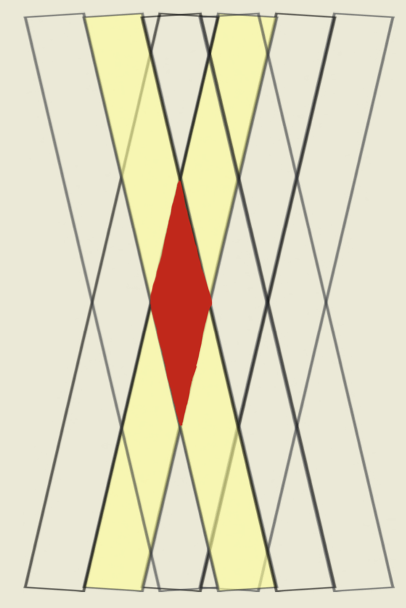
\includegraphics[height=5.0cm]{img/igata_01.png}
    \caption{1層分のシンチレータ}
    \label{fig:igata01}
\end{figure}
\subsection{ヒット情報作成の問題点}
\ref{subsec:anal:make_hit}節で説明したヒット情報の計算方法には問題点が存在する。
1層に2個以上の荷電粒子が通過した場合に作成されたヒット情報からは飛跡を再構成できないという点である。
例えば, 図に示すようにシンチレータから得られたADC valueがしきい値を超えた場合は赤く塗られる箇所(荷電粒子が通過したと考えられる場所)が余分にできてしまい, 荷電粒子の本当の飛跡がわからなくなってしまう。本実験では光生成反応を探索しているため探索対象は複数の粒子の飛跡であるが, この問題点は複数の粒子の飛跡の再構成を難しくしてしまっている。

\section{光生成反応イベントの探索}